\section{SELECT statements and prompts}
\begin{itemize}
    \item Find all employees:
        \begin{minted}[autogobble]{sql}
            SELECT * FROM employee;
        \end{minted}
        \begin{figure}[H]
            \centering
            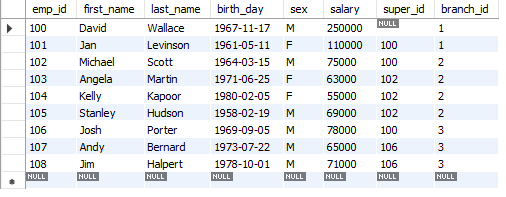
\includegraphics[width=0.4\textwidth]{./Figs/2020-12-24-20-38-38.png}
        % 	\caption{}
        \end{figure}
    
    \item Find all the clients:
        \begin{minted}[autogobble]{sql}
            SELECT * FROM client;
        \end{minted}
        \begin{figure}[H]
            \centering
            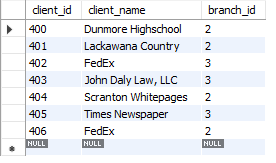
\includegraphics[width=0.4\textwidth]{./Figs/2020-12-24-20-39-09.png}
        % 	\caption{}
        \end{figure}
    
    \item Find all employees ordered by salary:
        \begin{minted}[autogobble]{sql}
            SELECT * FROM employee ORDER BY salary; 
        \end{minted}
        \begin{figure}[H]
            \centering
            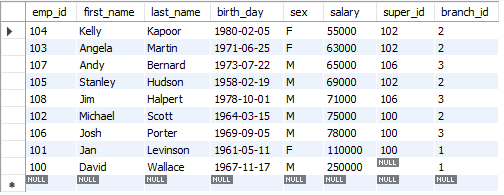
\includegraphics[width=0.4\textwidth]{./Figs/2020-12-24-20-39-36.png}
        % 	\caption{}
        \end{figure}
    
    \item Find all employees ordered by salary from largest to smallest and then smallest to largest:
        \begin{minted}[autogobble]{sql}
            SELECT * FROM employee ORDER BY salary DESC;
        \end{minted}
        \begin{figure}[H]
            \centering
            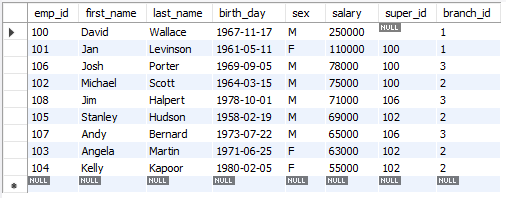
\includegraphics[width=0.4\textwidth]{./Figs/2020-12-24-20-44-00.png}
        % 	\caption{}
        \end{figure}
        \begin{minted}[autogobble]{sql}
            SELECT * FROM employee ORDER BY salary ASC;
        \end{minted}
        \begin{figure}[H]
            \centering
            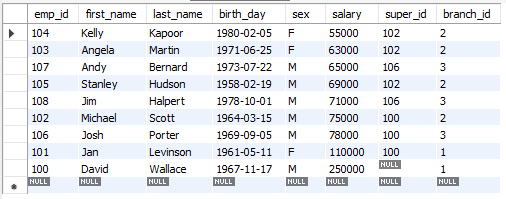
\includegraphics[width=0.4\textwidth]{./Figs/2020-12-24-20-44-41.png}
        % 	\caption{}
        \end{figure}
    
    \item Order all employees ordered by sex and then name:
        \begin{minted}[autogobble]{sql}
            SELECT * FROM employee ORDER BY sex, first_name, last_name; 
        \end{minted}
        \begin{figure}[H]
            \centering
            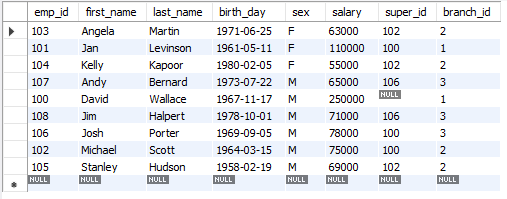
\includegraphics[width=0.4\textwidth]{./Figs/2020-12-24-20-43-11.png}
        % 	\caption{}
        \end{figure}
    
    \item Find the first 5 employees in the table:
        \begin{minted}[autogobble]{sql}
            SELECT * FROM employee LIMIT 5;
        \end{minted}
        \begin{figure}[H]
            \centering
            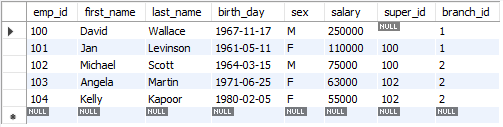
\includegraphics[width=0.4\textwidth]{./Figs/2020-12-24-20-45-25.png}
        % 	\caption{}
        \end{figure}
    
    \item Find the first and last names of all employees:
        \begin{minted}[autogobble]{sql}
            SELECT first_name, last_name FROM employee;
        \end{minted}
        \begin{figure}[H]
            \centering
            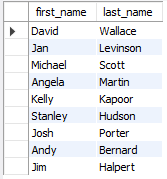
\includegraphics[width=0.4\textwidth]{./Figs/2020-12-24-20-45-46.png}
        % 	\caption{}
        \end{figure}
    
    \item  Find the forename and surnames of all employees:
        \begin{minted}[autogobble]{sql}
            SELECT first_name AS forename, last_name AS surname FROM employee;
        \end{minted}
        \begin{figure}[H]
            \centering
            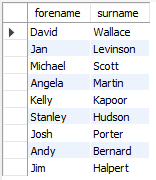
\includegraphics[width=0.4\textwidth]{./Figs/2020-12-24-20-46-18.png}
        % 	\caption{}
        \end{figure}
        \begin{itemize}
            \item \mintinline{sql}{AS} Allows you to select the columns differently to their names.
        \end{itemize}
    
    \item Find out all the different genders:
        \begin{minted}[autogobble]{sql}
            SELECT  DISTINCT sex FROM employee;
        \end{minted}
        \begin{figure}[H]
            \centering
            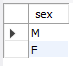
\includegraphics[width=0.4\textwidth]{./Figs/2020-12-24-20-46-37.png}
        % 	\caption{}
        \end{figure}
        \begin{itemize}
            \item \mintinline{sql}{DISTINCT} allows you to know all the values stored in a column. 
        \end{itemize}
    
    \item Find all male employees:
        \begin{minted}[autogobble]{sql}
            SELECT * FROM employee WHERE sex = 'M';
        \end{minted}
        \begin{figure}[H]
            \centering
            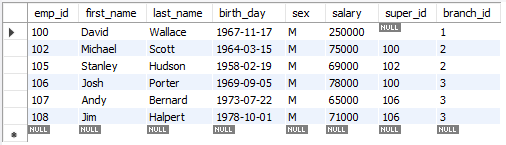
\includegraphics[width=0.4\textwidth]{./Figs/2020-12-24-20-47-19.png}
        % 	\caption{}
        \end{figure}
    
    \item Find all employees at branch 2:
        \begin{minted}[autogobble]{sql}
            SELECT * FROM employee WHERE branch_id = 2;
        \end{minted}
        \begin{figure}[H]
            \centering
            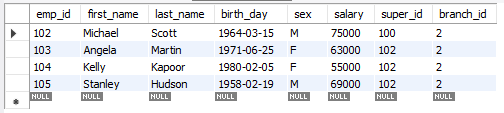
\includegraphics[width=0.4\textwidth]{./Figs/2020-12-24-20-48-13.png}
        % 	\caption{}
        \end{figure}
    
    \item Find all employee's id's and names who were born after 1969:
        \begin{minted}[autogobble]{sql}
            SELECT emp_id, first_name, last_name FROM employee WHERE birth_day >= 1970-01-01;
        \end{minted}
        \begin{figure}[H]
            \centering
            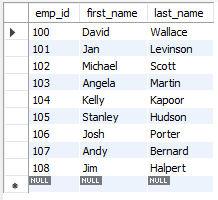
\includegraphics[width=0.4\textwidth]{./Figs/2020-12-24-20-48-48.png}
        % 	\caption{}
        \end{figure}
    
    \item Find all female employees at branch 2:
        \begin{minted}[autogobble]{sql}
            SELECT * FROM employee WHERE branch_id = 2 AND sex = 'F';
        \end{minted}
        \begin{figure}[H]
            \centering
            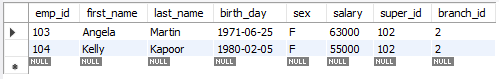
\includegraphics[width=0.4\textwidth]{./Figs/2020-12-24-20-49-50.png}
        % 	\caption{}
        \end{figure}
    
    \item Find all employees who are female  \& born after 1969 or who make over 80000:
        \begin{minted}[autogobble]{sql}
            SELECT * FROM employee WHERE (birth_day >= '1970-01-01' AND sex = 'F') OR salary > 80000;
        \end{minted}
        \begin{figure}[H]
            \centering
            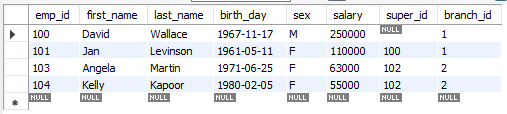
\includegraphics[width=0.4\textwidth]{./Figs/2020-12-24-20-50-39.png}
        % 	\caption{}
        \end{figure}
    
    \item Find all employees born between 1970 and 1975:
        \begin{minted}[autogobble]{sql}
            SELECT * FROM employee WHERE birth_day BETWEEN '1970-01-01' AND '1975-01-01';
        \end{minted}
        \begin{figure}[H]
            \centering
            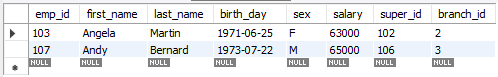
\includegraphics[width=0.4\textwidth]{./Figs/2020-12-24-20-51-24.png}
        % 	\caption{}
        \end{figure}
    
    \item Find all employees named Jim, Michael, Johnny or David:
        \begin{minted}[autogobble]{sql}
            SELECT * FROM employee WHERE first_name IN ('Jim', 'Michael', 'Johnny', 'David');
        \end{minted}
        \begin{figure}[H]
            \centering
            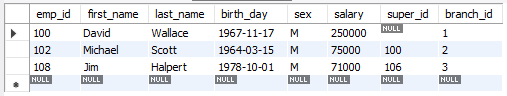
\includegraphics[width=0.4\textwidth]{./Figs/2020-12-24-20-52-10.png}
        % 	\caption{}
        \end{figure}
\end{itemize}

